% UPDATED BY MARCUS SCHAGERBERG, 2023
% CREATED BY WOLFGANG AHRENDT, 2021

\section{Tools}

% WRITTEN BY JAKOB WINDT, 2023
\subsection{Unity}

The simulation tool is built in a well-known game-engine software called Unity. There are a few reason why it was chosen as the development platform for the project instead of a similar game-engine like Unreal Engine. To begin with, C\# is the main programming language supported by Unity, which some of the team members had previous experience with. Furthermore, C\# is a higher level language compared to C++, the main language of Unreal Engine, making it easier for the team members without experience to learn. Because of this, the time it took to begin programming in the early stages of the project was most likely shorter, compared to if Unreal Engine was chosen as the platform.
\\\\
Another reason would be that Unity comes with the Unity Asset Store, a marketplace for acquiring creator made assets. This feature is important because, for example, instead of having to create custom models for the vehicles, they could instead be purchased using the given budget. This saves a lot of time, that could be better spent on other parts of the project. One of the more notable purchased assets is Edy's Vehicle Physics that are used to rig vehicle models with realistic physics. Instead of having to develop custom vehicle physics for each model, the team could instead use the asset to quickly configure a model with physics.
\\\\
% NOTE: need to find out why
The final and most important reason is why Unity was chosen, is because of its flexible developing structure. 

% WRITTEN BY JAKOB WINDT, 2023
\subsection{GitHub}

A commonly used tool when developing software in larger groups is Git. Git is a free and open-source version control system that allows its users to collaborate in a efficient and easy way. 
\\\\
GitHub is an online software development platform that utilizes Git to store and track software projects. It allows for users to work in their own separate branches, and later merge those into the main repository. Before a team member could merge their new code to the main repository, the code would have to be reviewed by at least one other team member to ensure that the code was well commented, functional, and that it follow the C\# coding standard.

% WRITTEN BY JAKOB WINDT, 2023
\subsection{Trello}

It was decided early on that the projects work flow should follow the SCRUM and Agile software development practices. Trello is a website that hosts scrum-boards in an user-friendly way. This allowed the team to keep track of what needs to be worked on in the project during the sprints. A sprint is a set time period when new tickets are made, and completed.

% WRITTEN BY JAKOB WINDT, 2023
\subsection{Balsamiq Wireframes}

During the first stage of creating a UI, its important to start with a simple mock-up design. This is what the tool, Balsamiq Wireframes, is used for. The user can quickly design wire frames depicting how the UI will appear during different times in the program. This includes everything from buttons to pop-up menu's that might appear in the simulation tool.

\section{Simulation Design and Implementation}

\subsection{ABM}

\subsection{Road Generation}

\subsection{City Generation}

% WRITTEN BY HANNES KAULIO, 2023
\subsection{Navigation}
The basic navigational responsibility of each agent is to be able to follow the road lanes, avoid colliding into other agents or buildings, follow the traffic rules and being able to navigate to a given position.
\\\\
This behavior is achieved by creating a navigation path for each road lane. The path is created as a double linked list. The nodes are insert along the lanes Bézier curve at a constant rate. Each node on the linked list store all information needed to navigate that lane. The position of the node, the agent that is currently on the node and special traffic rules the vehicles need to follow are stored on the node. Traffic signs such as stop sign are represented as a node and the traffic logic can be accessed by the agent when they encounter the node.
\\\\

% TODO write about snocks
snocks



To enable the ability to navigate the roads, a weighted directed graph is created from the road system.
The graph nodes are all the road endpoints and intersections. The edges between the nodes are weighted with a cost that is calculated as the distance * the speed limit.
The agents navigate to a given end node by receiving a path of nodes from the A* algorithm. When an agent drives up to a intersection, the intersections give a new road path to follow given the navigation node the agent is traveling to.


\section{Graphics}

\subsection{Third-Party Assets}

\subsection{Animations}

\subsection{Environment Materials and Textures}



\section{Performance}

\subsection{Quality vs Performance}

\subsection{Performance Benchmarks}


% WRITTEN BY MARTIN BLOM, 2023
\section{Work flow}
When developing any software larger than just a single use script, the amount of work and information can quickly grow beyond the level of ones own simultaneous comprehension. Therefore these kinds of projects require rigorous planning and strategizing to not get lost in all the different tasks and do them in a smooth and reasonable order, that allows for parallel continuous progress.
\\\\
To achieve this a strict work flow framework was developed, where the first step was to analyze the work load and disposable time. This included drafting a time plan for the whole time scope of the project \ref{fig:time-plan}. 

\begin{figure}[H]
    \centering
    \fbox{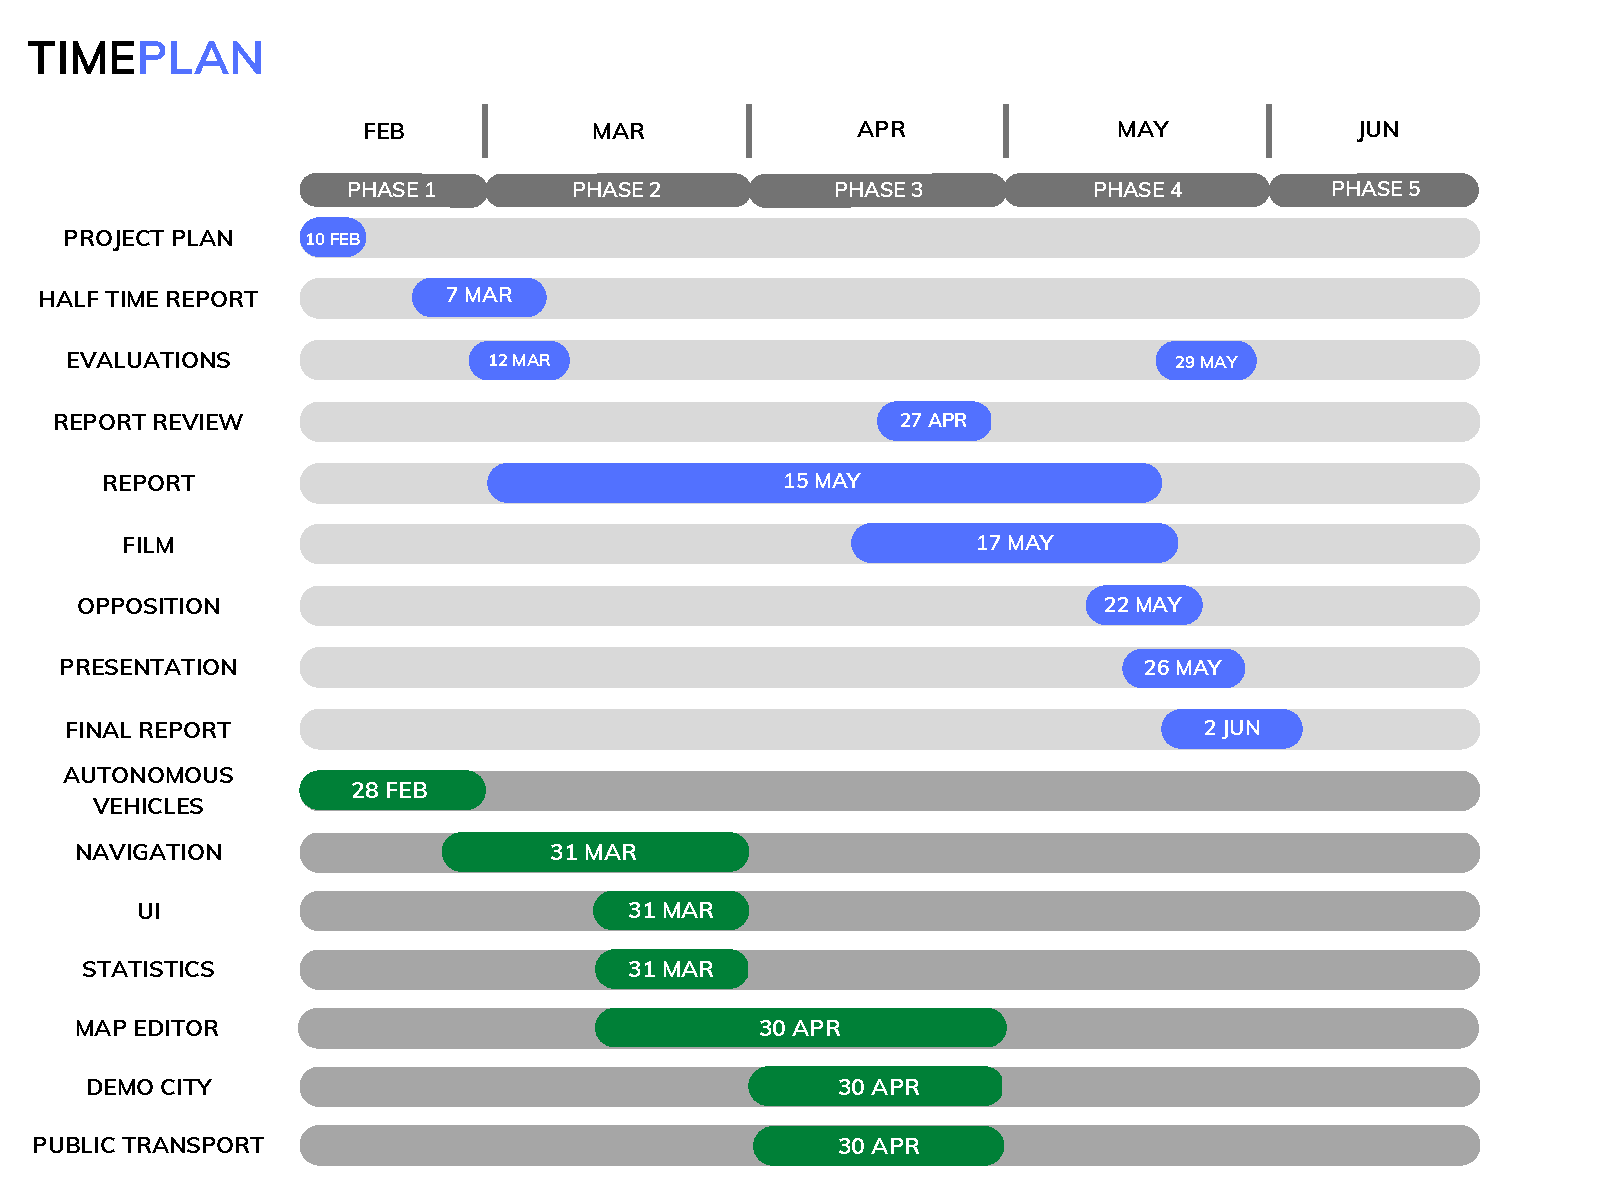
\includegraphics[scale=0.5]{Project_report/appendix/Time_plan.pdf}}
    \caption{Project Time Plan}
    \label{fig:time-plan}
\end{figure}

With this it's now much easier to keep track of the general progress of the project, as well as helping with planning short term goals. Coincidentally this is the next step of the work flow model. The short term goals where planned using a scrum framework with weekly sprints, explained in \ref{sub:weekly-sprints}. These sprints were upheld for the duration of the project to keep a stead flow of progress, together with the time plan they create a very clear way of seeing the current state of completeness. 
\\\\
The third aspect of the work flow is the approval of progress. As mentioned earlier a large project requires a substantial amount of planning to not get lost. The approval of progress can be seen as just as important as the planning and execution itself. Without a popper method of approving new advancements/functionality, the project can quickly falter. If progress never goes through the process of approval many things can go wrong. Evidently, badly written code can cause issues that are easily preventable with a quick inspection. Code can even be considered good but with no input from the rest of the team, visions of how higher order elements will be implemented can differ. This can implicitly create  more complex problems much further on, which can be very hard and time consuming to resolve. To solve this, code review's \ref{sub:code-reviewing} for every change made are part of the work flow.  

\subsection{Weekly Sprints} \label{sub:weekly-sprints}
The weekly sprint model stems from the scrum framework, which is a framework for developing and sustaining complex products. The sprint model follows 4 repeating stages of development: Planning, Implementation, Review and Retrospect.
\\\\
Each sprint starts out in the planning stage, where a meeting is held to set up this sprints goals. This includes moving/creating stories for the backlog as well as the current sprint. The stories are mainly chosen by the project manager then developed in unison with the scrum master and input from the rest of the team.
\\\\
The next stage of the sprint is the implementation itself. This is the time were the teams focus is solely on delivering good quality solutions to complete all of the current sprints stories, and eventually working on the backlog as time is presented.
\\\\
Next up is the review stage, not to be confused with code reviewing \ref{sub:code-reviewing}. In this stage another meeting is held called a "Demo meeting", where all members get to do a small demonstration of all their progress during the sprint. This is an important step to onboard all members on new functionality and make sure that desired behaviour is achieved. When a story is regarded as fully complete it's archived to make room for new ones.
\\\\
Lastly the retrospect stage, which is usually carried out following the review stage. In the retrospect stage the current sprints efficiency and quality is discussed. And plans/ways to increase these and the overall effectiveness are considered. When all is done the cycle begins anew until the project is done.

\subsection{Code Reviewing} \label{sub:code-reviewing}
% TODO 
% describe code review process

\section{Testing}